\chapter{Implementación y pruebas del prototipo}
\ihead[]{Capítulo 7: Implementación del prototipo}
\label{ch:CH07}
%%%%%%%%%%%%%%%%%%%%%%%%%%%%%%%%%%%%%%%%%%

\noindent
En este capítulo se recopilan las pruebas realizadas con un prototipo, con el objetivo de validar el funcionamiento del diseño electrónico y mecánico, así como del \ac{SW}, para lograr una implementación correcta de la solución general planteada en los Capítulos~\ref{ch:CH04}, \ref{ch:CH05} y \ref{ch:CH06}. En primer lugar, se presentan las pruebas y configuraciones de los componentes que conforman el \ac{HW}, empleando elementos de prototipado rápido, como piezas fabricadas mediante impresión 3D y placas perforadas para el montaje electrónico. En cuanto al \ac{SW} de la solución, se muestran fragmentos representativos del código, con énfasis en la lógica de recepción y envío de datos.
\section{Desarrollo de la tarjeta}

\noindent
Con el objetivo de acelerar la validación experimental del sistema, en esta etapa se emplea una placa de pruebas en lugar de la \ac{PCB} diseñada en el Capítulo~\ref{ch:CH04}. Esta decisión permite prototipar e iterar rápidamente sobre los valores de los componentes dimensionados en dicho capítulo, facilitando ajustes durante las primeras pruebas de funcionamiento. Aun cuando la implementación física se realiza sobre una placa de pruebas, se mantienen los mismos pines y conexiones definidos en el Capítulo~\ref{ch:CH04}, de modo que la migración posterior a la \ac{PCB} no implique cambios en la asignación de señales.

\noindent
Asimismo, esta configuración permite validar la comunicación del microcontrolador con la interfaz de operación del sistema, así como verificar el desempeño de los bloques principales de sensado y actuación. En particular, tal como se observa en la Figura~\ref{fig:pcb_pruebas_prototipo}, se implementan los componentes más relevantes para la etapa de pruebas: el sensor de efecto Hall y el \textit{driver} para el control de los motores que serán sensados. En las siguientes secciones se detalla el funcionamiento de la placa de pruebas diseñada para la implementación del prototipo.

% ---------------------------------------------------------
% INSERTAR FIGURA: placa de pruebas del prototipo
% ---------------------------------------------------------
\begin{figure}[H]
  \centering
  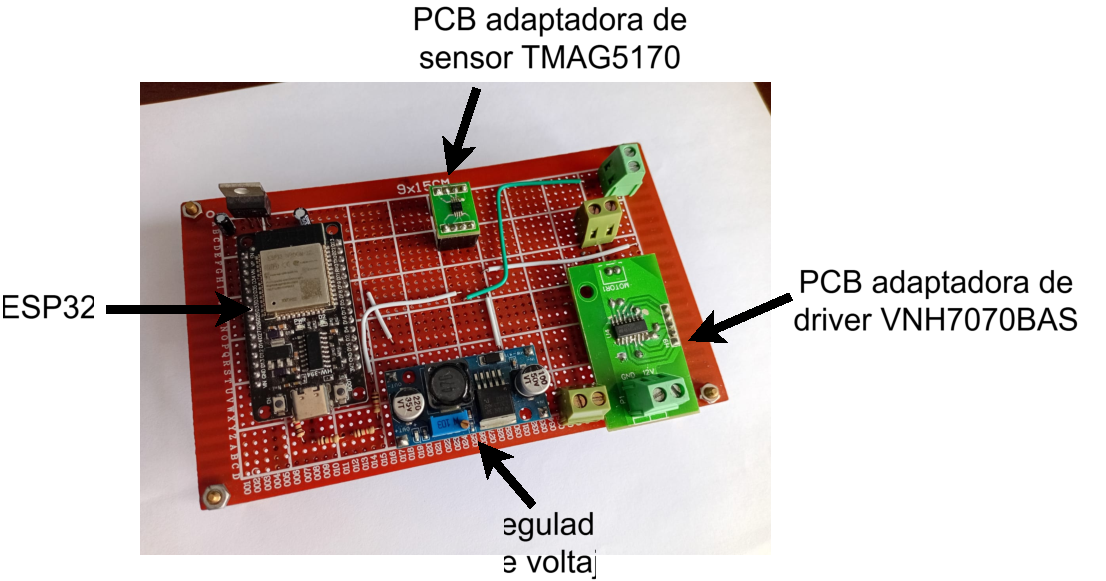
\includegraphics[width=0.90\linewidth]{CHPTRS/CH07_IMPLEMENTACION/Fig/hw_total_partes.pdf}
  \caption{Placa de pruebas diseñada para la implementación del prototipo.}
  \label{fig:pcb_pruebas_prototipo}
\end{figure}


\section{Prueba del sensor Hall}
\label{sec:prueba_sensor_hall}

\noindent
En esta sección se presentan las pruebas realizadas para la configuración del sensor de efecto Hall TMAG5170A1. Se muestran los componentes utilizados durante el montaje de prueba, los registros que deben editarse para su configuración y, finalmente, los resultados obtenidos en las pruebas realizadas con este sensor.

\subsection{Configuración mínima del TMAG5170A1 para detección de giro en el plano \(XY\)}

\noindent
Para las pruebas del sensor se empleó una \ac{PCB} de pruebas, mostrada en la Figura~\ref{fig:tmag_pcb_poc}, cuya finalidad es facilitar la integración del integrado en una placa de pruebas y permitir su conexión adecuada al microcontrolador. La implementación del montaje se muestra en la Figura~\ref{fig:tmag_pcb_poc}. Asimismo, se procuró validar cada componente y su circuito asociado de manera incremental, siguiendo los diseños presentados previamente en el Capítulo~\ref{ch:CH04}. La implementación del montaje se muestra en la Figura~\ref{fig:tmag_pcb_poc}. Para estas pruebas se procuró validar cada componente junto con su circuito asociado, previamente diseñado en el Capítulo~\ref{ch:CH04}.
 % ---- Figura: izquierda EasyEDA / derecha implementación ----
    % Requiere: \usepackage{subcaption}

\begin{figure}[H]
  \centering

  \begin{subfigure}[t]{0.48\textwidth}
    \centering
    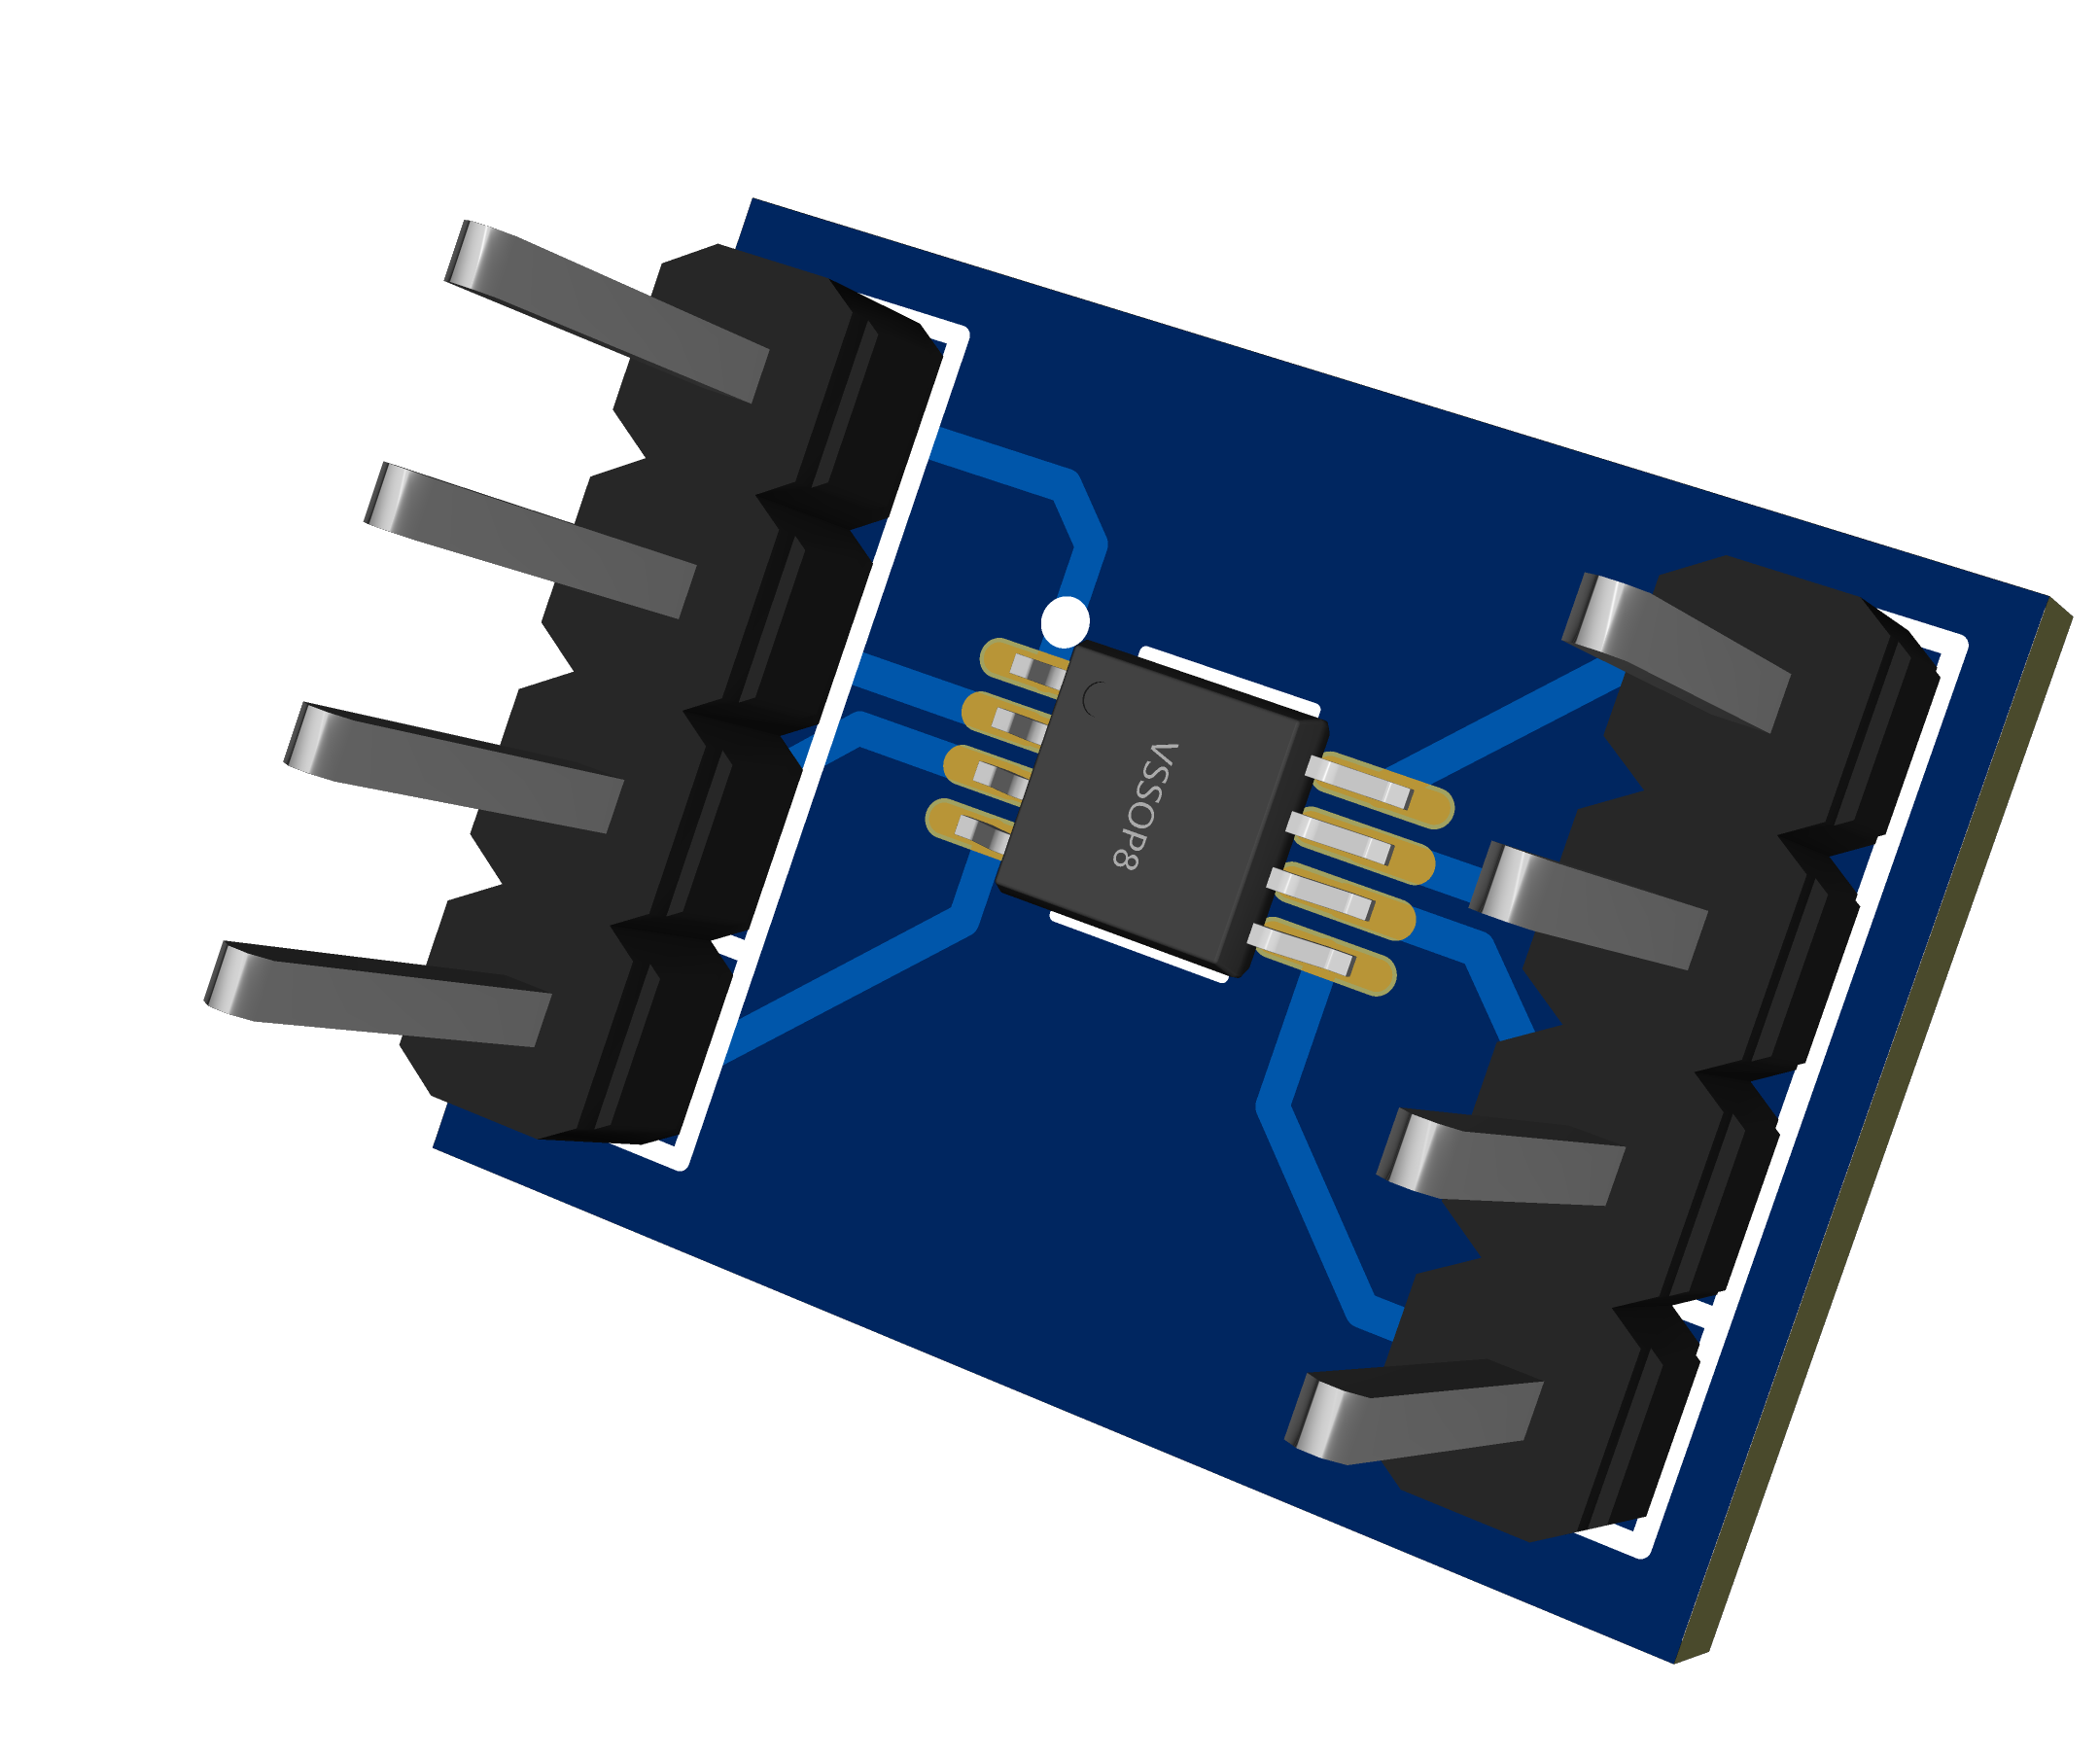
\includegraphics[width=\linewidth]{CHPTRS/CH07_IMPLEMENTACION/Fig/3D_PCB_TMAG.png}
    \caption{Diseño de la \ac{PCB} en EasyEDA.}
    \label{fig:diseñoPCBadapctacion}
  \end{subfigure}
  \hfill
  \begin{subfigure}[t]{0.48\textwidth}
    \centering
    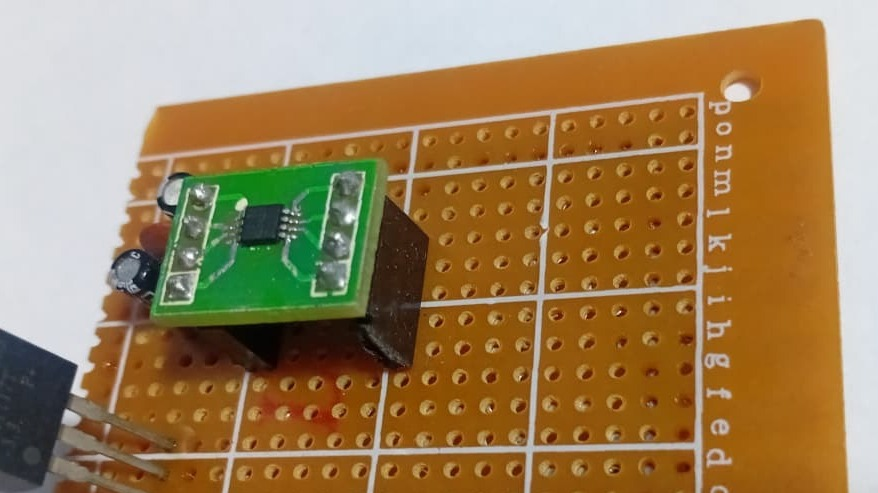
\includegraphics[width=\linewidth]{CHPTRS/CH07_IMPLEMENTACION/Fig/TMAG5170.jpeg}
    \caption{Implementación de la \ac{PCB} para pruebas.}
    \label{fig:implementacionsensor}
  \end{subfigure}

  \caption{\ac{PCB} para pruebas y configuración del sensor TMAG5170.}
  \label{fig:tmag_pcb_poc}
  \caption*{\footnotesize\textit{Nota: Componentes cortesía del profesor Enrique Vidal.}}
\end{figure}

\noindent
En este montaje se utiliza un regulador de \(3.3\,\text{V}\), el cual alimenta al sensor con el mismo nivel de tensión lógica que el microcontrolador ESP32. Para las pruebas se utilizó un módulo de desarrollo de este microcontrolador, el cual también será empleado  en la solución final.


\noindent
Según lo presentado en la Tabla~\ref{tab:pines_pcb}, se seleccionaron los pines 18, 19, 23 y 22 para la comunicación \ac{SPI} con el sensor (SCK, MISO, MOSI y CS, respectivamente). La configuración mínima del TMAG5170A1 se realizó mediante la escritura de registros internos. En particular, se deshabilitó el cálculo de CRC a través del registro de prueba y se habilitaron los canales \(X\), \(Y\) y \(Z\) con un rango de medición de \(\pm 100\,\text{mT}\), manteniendo el sistema en una configuración base para el sensado.

\noindent
En la Tabla~\ref{tabla_registros_tmag} se resumen los registros editados y los valores asignados en hexadecimal.

% ---------------------------------------------------------
% Tabla de registros configurados
% ---------------------------------------------------------
\begin{longtblr}[
  theme=pucp,
  label   = {tabla_registros_tmag},
  caption = {Registros configurados del TMAG5170A1 para sensado y estimación de ángulo en \(XY\).},
]{
  width=\linewidth,
  colspec = {Q[l,m,wd=0.30\linewidth] X[l,m] Q[c,m,wd=0.18\linewidth]},
  colsep=2pt,
  rowsep=1pt,
  rows={font=\footnotesize},
  row{1}={font=\footnotesize\bfseries,halign=c},
  rowhead=1, rowfoot=0,
  hlines, vlines,
}
Registro &
Descripción &
Valor escrito (hex) \\

\texttt{REG\_TEST\_CONFIG} \texttt{(0x0F)} &
Registro de prueba; se deshabilita CRC en la comunicación \ac{SPI} durante la etapa de pruebas. &
\texttt{0x000407} \\

\texttt{REG\_DEVICE\_CONFIG} \texttt{(0x00)} &
Configuración general del dispositivo; en esta prueba se habilita el modo de medición activo. &
\texttt{0x0020} \\

\texttt{REG\_SENSOR\_CONFIG} \texttt{(0x01)} &
Configuración del sensor; habilita los ejes \(X\), \(Y\) y \(Z\) y define el rango de medición del campo magnético. &
\texttt{0x41EA} \\

\texttt{REG\_SYSTEM\_CONFIG} \texttt{(0x02)} &
Configuración del sistema; para esta prueba mínima se mantiene el valor base. &
\texttt{0x0000} \\

\end{longtblr}

\noindent
Una vez aplicada la configuración, se realizó la lectura de los registros de resultado de \(X\), \(Y\) y \(Z\). Con estas mediciones se calculó el ángulo en el plano \(XY\) mediante \(\theta=\mathrm{atan2}(Y,X)\) y se ajustó su rango a \([0, 360]\,\text{grados}\). Para evitar discontinuidades al cruzar \(0/360^\circ\), se aplicó un ajuste de la variación angular para mantener la diferencia entre muestras dentro de \([-180,180]\) grados. Finalmente, la velocidad angular se obtiene como \(\omega=\Delta\theta/\Delta t\) y se convirtió a \(\text{rad}/\text{s}\).

\noindent
El sensor traduce la variación del campo magnético en una estimación de la posición angular en el eje solidario del motor. A partir de esta señal, se calcula la velocidad angular mediante la derivada temporal de la posición angular, como se muestra en la Figura~\ref{fig:graph_ang}.

% INSERTAR FIGURA: gráfica de ángulo y velocidad angular
\begin{figure}[ht!]
  \centering
  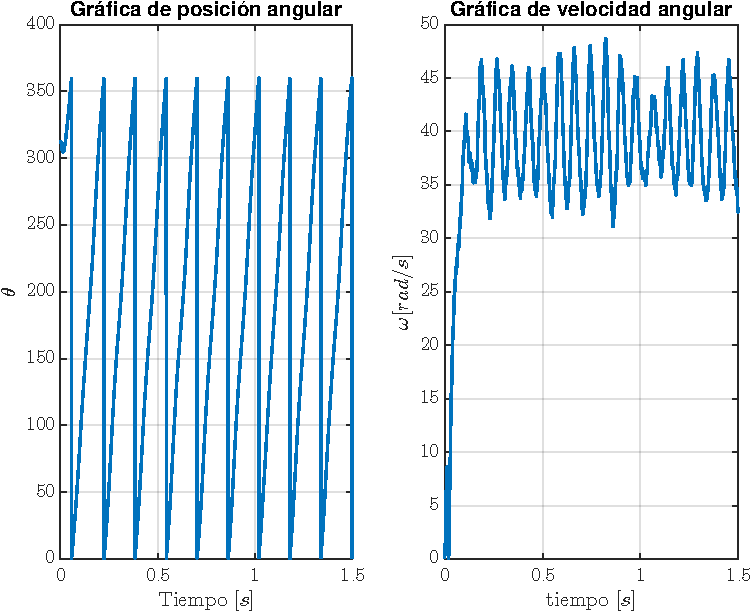
\includegraphics[width=0.95\linewidth]{CHPTRS/CH07_IMPLEMENTACION/Fig/ang_graph.pdf}
  \caption{Señales de posición angular y velocidad angular obtenidas a partir del TMAG5170A1.}
  \label{fig:graph_ang}
\end{figure}

\noindent
Para esta toma de datos no se utilizó ningún soporte mecánico, por lo que la señal de velocidad presenta ruido y no converge a un valor específico. Este comportamiento puede deberse a las vibraciones generadas durante la medición, principalmente por el movimiento de la mano al acercar el eje del motor con el imán hacia el sensor.
 
\section{Pruebas con el driver de motor}
\label{sec:pruebas_driver}

\noindent
Para las pruebas con el driver VNH7070BAS se empleó una etapa de potencia basada en el puente H seleccionado en el Capítulo~\ref{ch:CH04}, con el objetivo de validar su funcionamiento antes de integrarlo al prototipo final. En esta etapa se verificó la correcta excitación del motor \ac{DC} mediante señales de control provenientes de la ESP32 (habilitación, sentido de giro y \ac{PWM}), así como la lectura de la salida de sensado CS para su posterior adquisición por el ADC. Las pruebas se realizaron en un entorno de prototipado rápido, utilizando conexiones accesibles y puntos de medición que permiten observar las señales principales del driver y confirmar su compatibilidad con la lógica a \SI{3.3}{\volt} del microcontrolador.

% Requiere: \usepackage{subcaption}

\begin{figure}[H]
  \centering

  \begin{subfigure}[t]{0.48\textwidth}
    \centering
    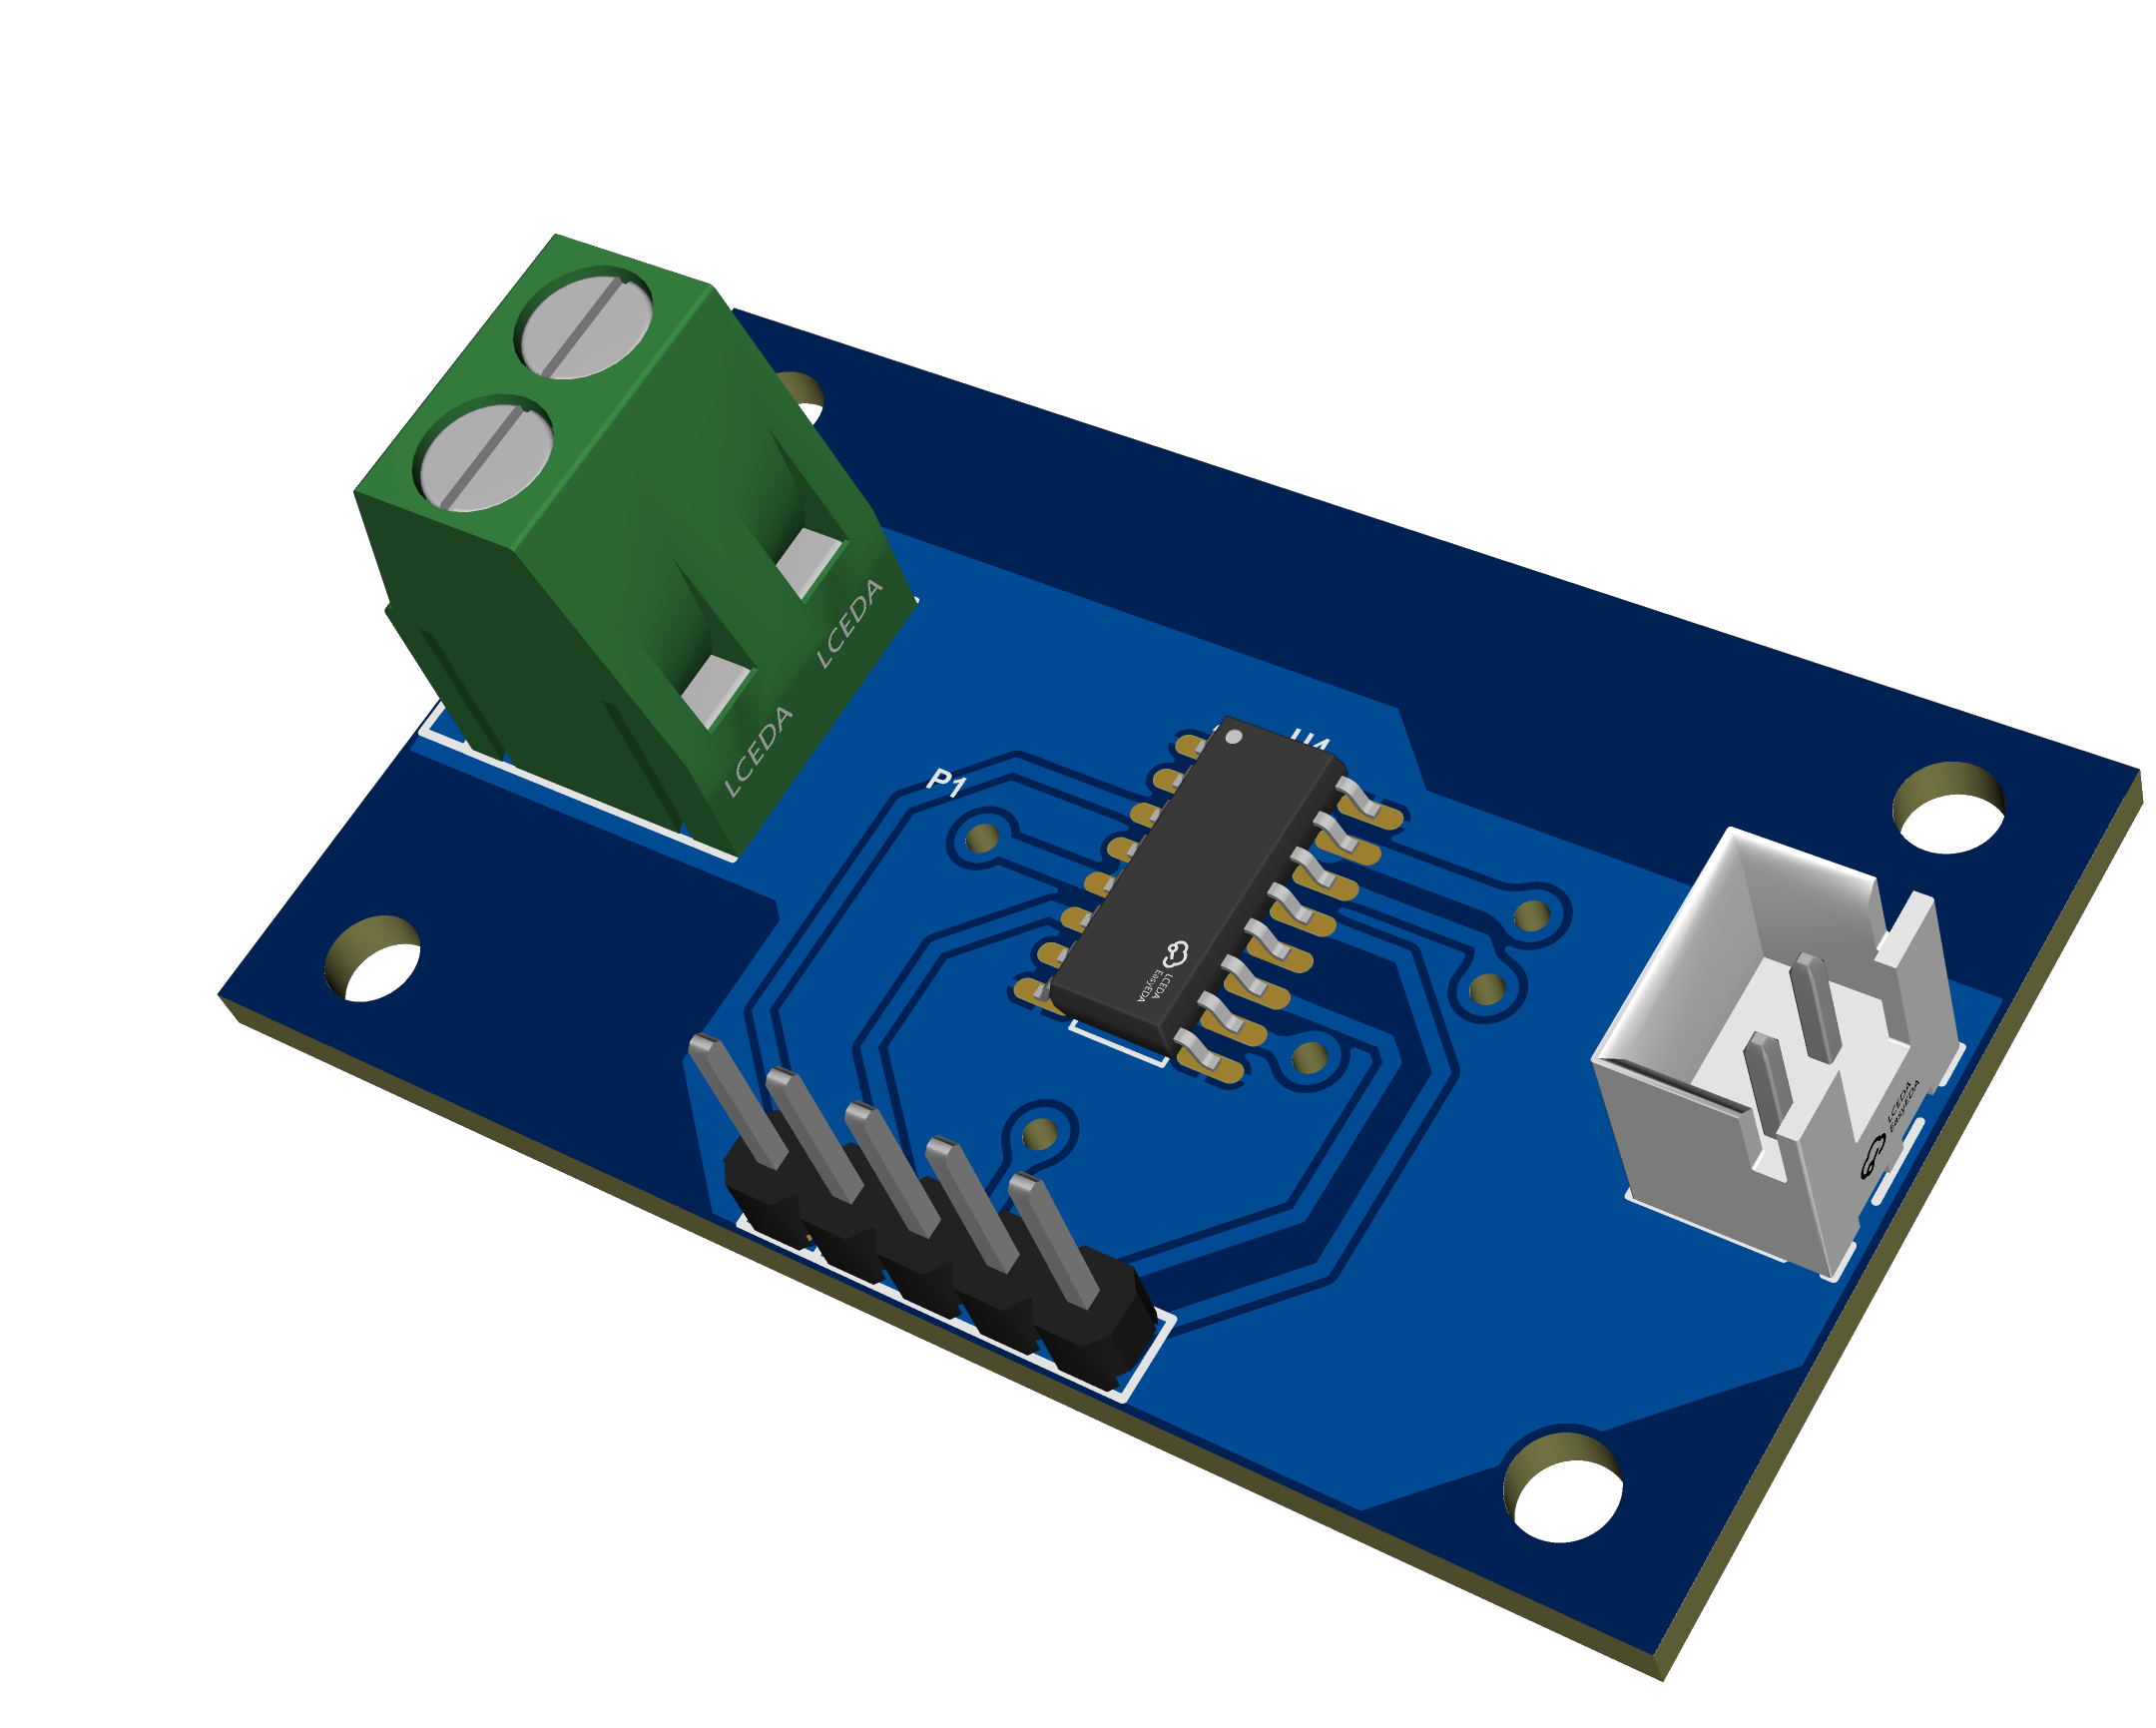
\includegraphics[width=\linewidth]{CHPTRS/CH07_IMPLEMENTACION/Fig/3D_PCB5_VNH.png}
    \caption{Diseño de la \ac{PCB} del driver VNH7070BAS en EasyEDA.}
    \label{fig:vnh_pcb_diseno}
  \end{subfigure}
  \hfill
  \begin{subfigure}[t]{0.48\textwidth}
    \centering
    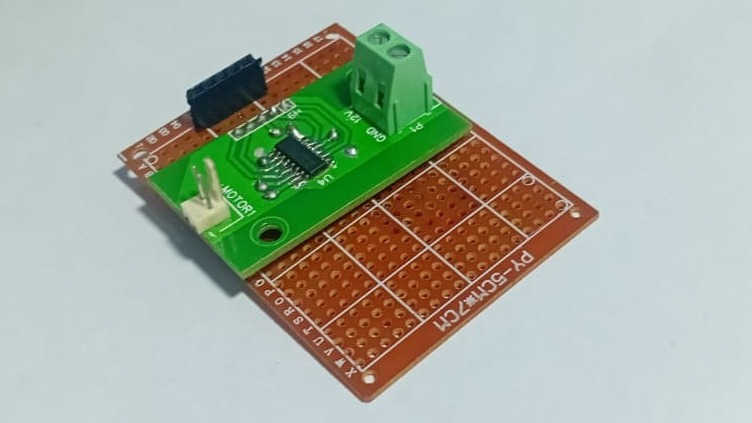
\includegraphics[width=\linewidth]{CHPTRS/CH07_IMPLEMENTACION/Fig/VNH.jpeg}
    \caption{Implementación física del \textit{driver} VNH7070BAS en una placa de pruebas.}
    \label{fig:vnh_pcb_impl}
  \end{subfigure}

  \caption{Implementación de prueba del \textit{driver} VNH7070BAS.}
  \label{fig:vnh_pcb_poc}
  \caption*{\footnotesize\textit{Nota: Componentes cortesía del profesor Enrique Vidal.}}
\end{figure}

\noindent
Una vez obtenida la \ac{PCB} de pruebas, se comenzó a realizar la conexión con los pines asignados para el control del driver del motor, con el objetivo de obtener los parámetros de voltaje y corriente que llegan al motor. Para la medición del voltaje del motor, se emplea un divisor de tensión conectado a la entrada del voltaje nominal. Esto se debe a que el microcontrolador seleccionado cuenta con un ADC que opera en el rango de \SIrange{0}{3.3}{\volt}. 
De manera similar a las pruebas del sensor Hall, se presentan los resultados del sensado de las variables medidas. En la Figura~\ref{fig:graph_voltaje} se muestra el registro de la tensión de la fuente de alimentación del motor, correspondiente a \SI{12}{\volt} nominal.

% ---------------------------------------------------------
% Figura: sensado de voltaje
% ---------------------------------------------------------
\begin{figure}[ht!]
\centering
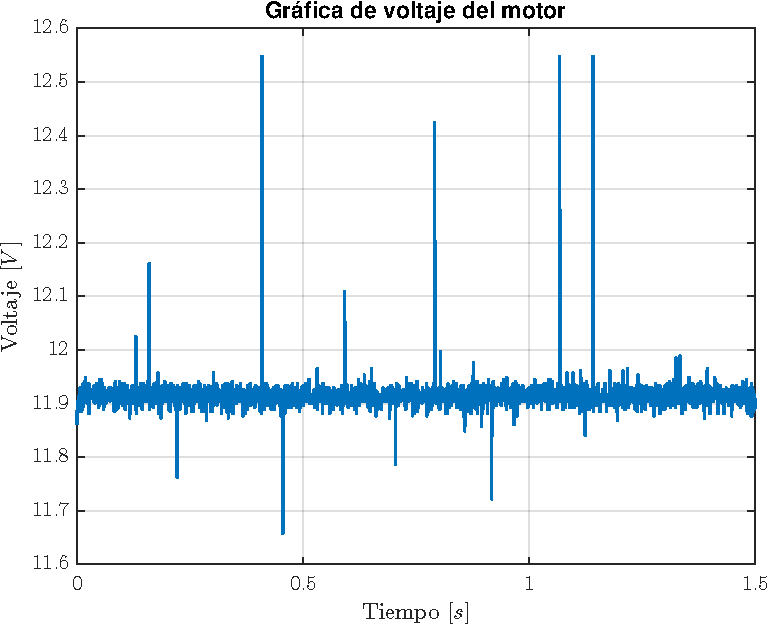
\includegraphics[width=0.70\linewidth]{CHPTRS/CH07_IMPLEMENTACION/Fig/voltaje_graph.pdf}
\caption{Señal de voltaje de alimentación del motor obtenida durante las pruebas.}
\label{fig:graph_voltaje}
\end{figure}

\noindent
En cuanto a la corriente, se presentan dos registros. Para estas pruebas, se diseñó el circuito de adecuación de señal de voltaje que permite medir la corriente de los motores evaluados; sin embargo, esta medición se realiza a partir de una ganancia de escalamiento $K$ que relaciona la corriente real del motor con la señal de sensado, la cual corresponde a un valor típico indicado en la hoja de datos \autocite{ST_VNH7070BAS}, tal como se describe en la sección \ref{sec:diseno_filtros_sensado} del Anexo \ref{an:Anexo_u}. Debido a que $K$ es un valor típico y puede variar según el motor sensado y sus parámetros eléctricos (por ejemplo, resistencia e inductancia), es necesario emplear una pinza amperométrica para validar experimentalmente que la corriente medida por el sistema corresponde a la corriente real del motor. En la Figura~\ref{fig:graph_current_start} se muestra la toma de datos durante \SI{1.5}{\second}, en la cual se observa un pico de corriente al inicio debido a la inercia asociada al arranque del motor. Por otro lado, en la Figura~\ref{fig:graph_current_forced} se presenta un lapso de tiempo más prolongado, en el cual se forzó el eje del motor con el propósito de verificar la coherencia de la medición; bajo esta condición se espera un incremento de corriente para vencer la fuerza que restringe el giro del eje. En ambos casos, también se aprecia el ruido presente en la señal de corriente, la cual es adquirida por el microcontrolador como una medición de voltaje.


% ---------------------------------------------------------
% Figura con dos subfiguras: corriente normal y corriente forzada
% ---------------------------------------------------------
%---------------------------------------------------------
% Figura: corriente durante arranque (1.5 s)
%---------------------------------------------------------
\begin{figure}[H]
\centering
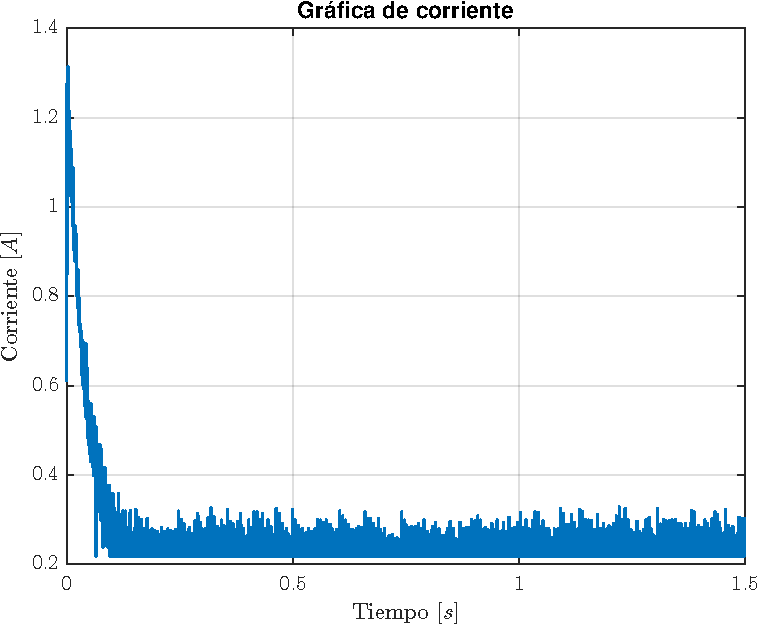
\includegraphics[width=0.80\linewidth]{CHPTRS/CH07_IMPLEMENTACION/Fig/corriente_graph.pdf}
\caption{Corriente durante el arranque del motor (\SI{1.5}{\second}).}
\label{fig:graph_current_start}
\end{figure}

%---------------------------------------------------------
% Figura: corriente con eje forzado
%---------------------------------------------------------
\begin{figure}[H]
\centering
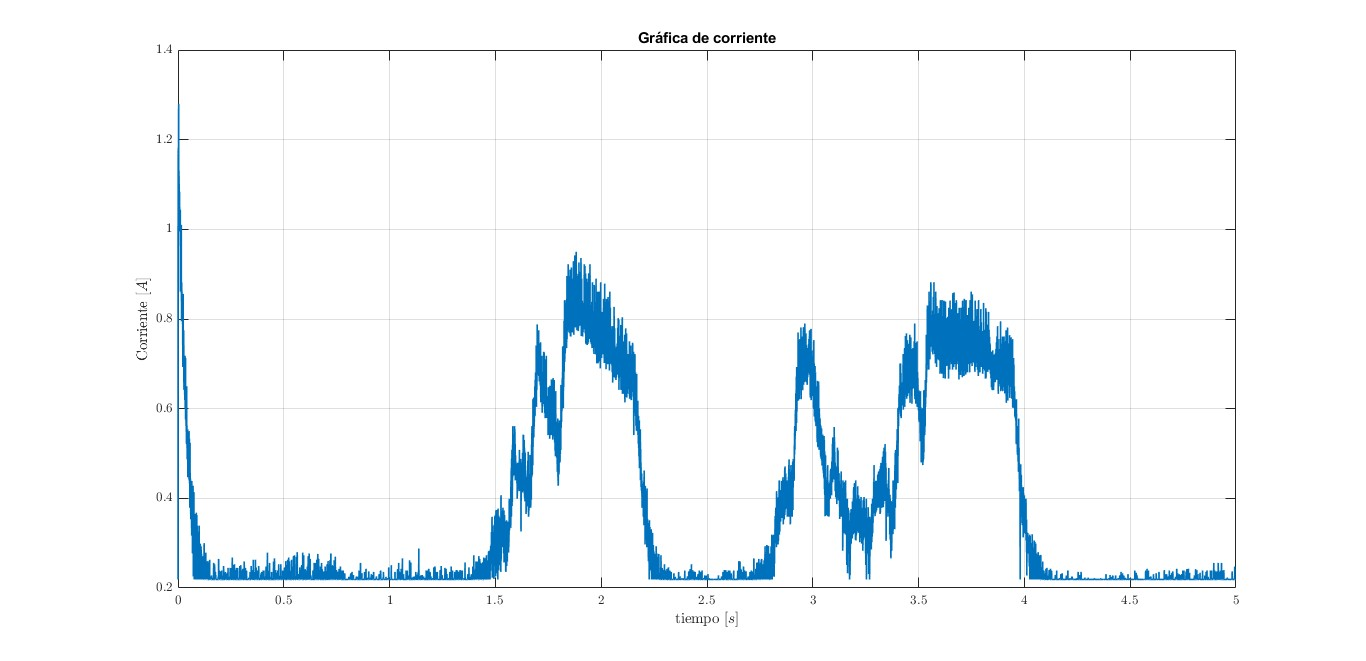
\includegraphics[width=\linewidth]{CHPTRS/CH07_IMPLEMENTACION/Fig/corriente_graph_force.jpg}
\caption{Corriente con eje forzado durante un intervalo prolongado.}
\label{fig:graph_current_forced}
\end{figure}

\noindent
Para todas estas pruebas, tanto de voltaje como de corriente y velocidad angular, se trabajó con un periodo entre muestras de \SI{500}{\micro\second}, lo que equivale a una frecuencia de muestreo de \SI{2}{\kilo\hertz}. Este muestreo busca capturar adecuadamente el arranque del motor en pruebas de corta duración, debido a que la dinámica de estas variables es rápida y converge en un intervalo reducido, tal como se observa en las figuras presentadas. Por este motivo, se optó por una ventana de adquisición de aproximadamente \SI{1.5}{\second}, donde la información es almacenada en la memoria RAM del microcontrolador para luego ser enviada hacia la interfaz, en la cual se ejecutará el algoritmo de estimación. Para mayor detalle sobre la lógica de funcionamiento del sistema, esta se describe en el Capítulo~\ref{ch:CH06}, correspondiente al desarrollo de la lógica de control y \ac{SW}.


\section{Prueba de sensado utilizando el \ac{HW} implementado}

\noindent
Con el objetivo de validar el banco de pruebas, se realizaron pruebas experimentales utilizando motores \ac{DC} comerciales de \SI{12}{V}. Llos motores que se probarán a continuación no cuentan con una ficha técnica. Es por ello, que la obtención de sus parámetros eléctricos y mecánicos deberá realizarse mediante comparación entre los métodos empíricos descritos en el Anexo \ref{an:Anexo_C} y el método de estimación paramétrica propuesto en este trabajo.
\noindent
Los motores utilizados corresponden a los modelos JGB37 y JGA25, cuya nomenclatura hace referencia al diámetro externo del cuerpo del motor (\SI{37}{mm} y \SI{25}{mm}, respectivamente), dimensión relevante para el diseño mecánico del sistema de acople. Ambos motores fueron montados sobre perfiles de aluminio V-SLOT utilizando un \textit{bracket} diseñado con su geometría específica para garantizar su sujeción en la toma de datos. A continuación, en la Figura \ref{fig:motores_prueba} se presentan las fotos con los motores mencionados sujetos al perfil.

\begin{figure}[!ht]
    \begin{tabularx}{\linewidth}{*{2}{>{\centering\arraybackslash}X}}
        % FILA-1 (IMÁGENES)
        \begin{subfigure}[t]{0.45\textwidth}
            \centering
            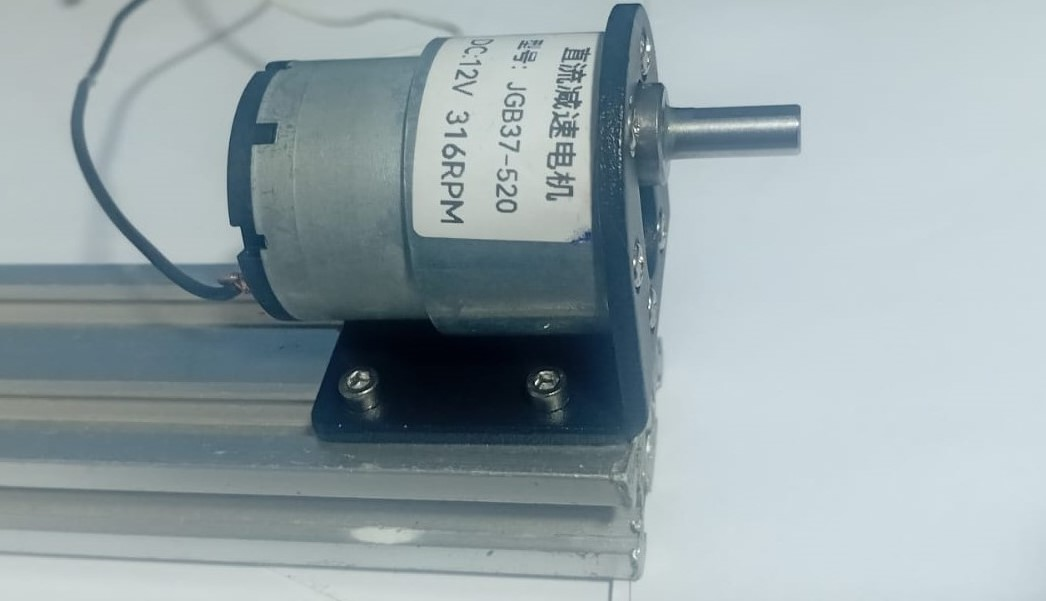
\includegraphics[width=.9\linewidth]{CHPTRS/CH07_IMPLEMENTACION/Fig/MotorGB37.jpeg}
        \end{subfigure}
        &
        \begin{subfigure}[t]{0.45\textwidth}
            \centering
            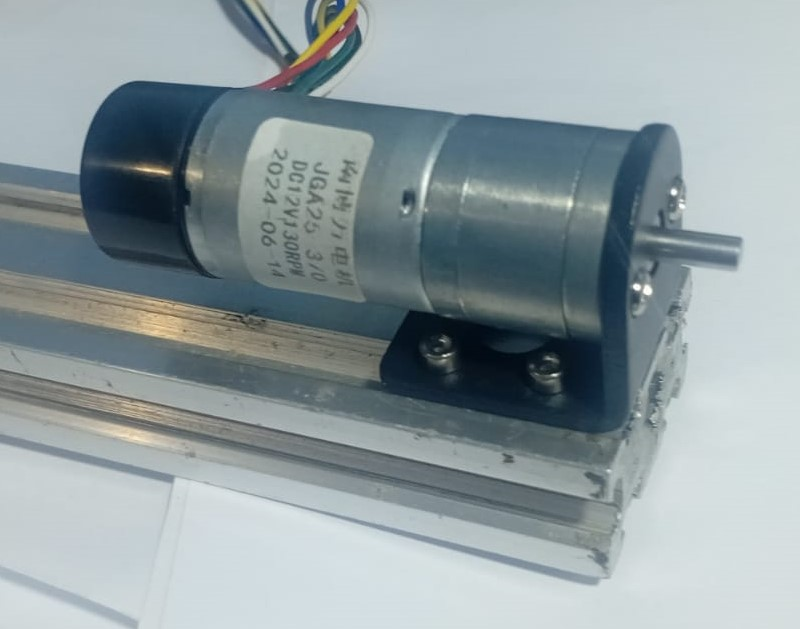
\includegraphics[width=.9\linewidth]{CHPTRS/CH07_IMPLEMENTACION/Fig/MOTORGA25.jpeg}
        \end{subfigure}
        \\ 
        % FILA-2 (CAPTIONS + LABELS)
        \begin{subfigure}[t]{0.9\linewidth}
            \caption{Motor \ac{DC} JGB37 de \SI{37}{mm} de diámetro, montado sobre perfil de aluminio mediante soporte impreso en 3D.}
            \label{fig:motor_jgb37}
        \end{subfigure}
        &
        \begin{subfigure}[t]{0.9\linewidth}
            \caption{Motor \ac{DC} JGA25 de \SI{25}{mm} de diámetro, acoplado al sistema de pruebas.}
            \label{fig:motor_jga25}
        \end{subfigure}
    \end{tabularx}
    \caption{Motores \ac{DC} utilizados para las pruebas experimentales de sensado.}
    \label{fig:motores_prueba}
\end{figure}
\noindent
Durante las pruebas iniciales se observó la necesidad de aplicar filtros para el tratamiento de los datos recolectados, especialmente en el sensado de la velocidad angular, debido a la presencia de ruido de medición y pequeñas oscilaciones por no haber sujetado correctamente el sensor de efecto \textit{hall}. En laa Figura \ref{fig:velocidades_prueba} se muestran los resultados de la medición de esta variable, que ejemplifica cómo es que influye que el imán de neodimio y el sensor estén lo más centrados posible.

\begin{figure}[!ht]
    \begin{tabularx}{\linewidth}{*{2}{>{\centering\arraybackslash}X}}
        % FILA-1 (IMÁGENES)
        \begin{subfigure}[t]{0.45\textwidth}
            \centering
            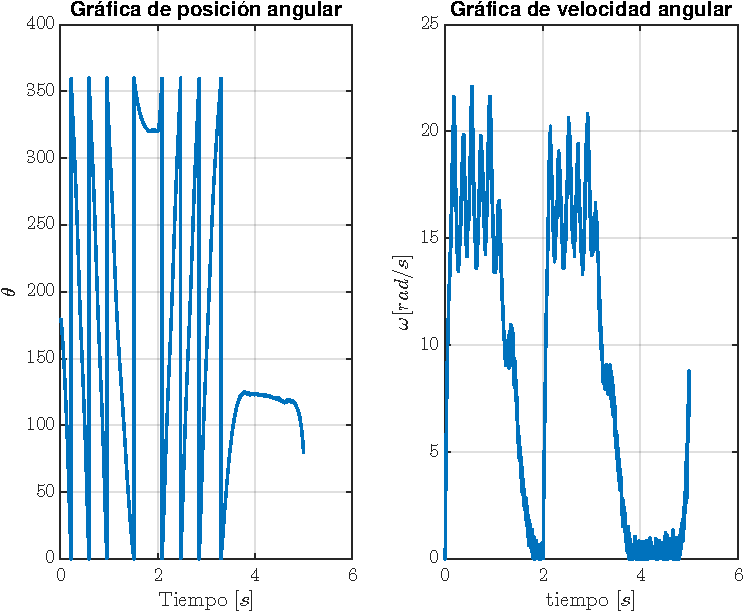
\includegraphics[width=.95\linewidth]{CHPTRS/CH07_IMPLEMENTACION/Fig/w_JGB37.pdf}
        \end{subfigure}
        &
        \begin{subfigure}[t]{0.45\textwidth}
            \centering
            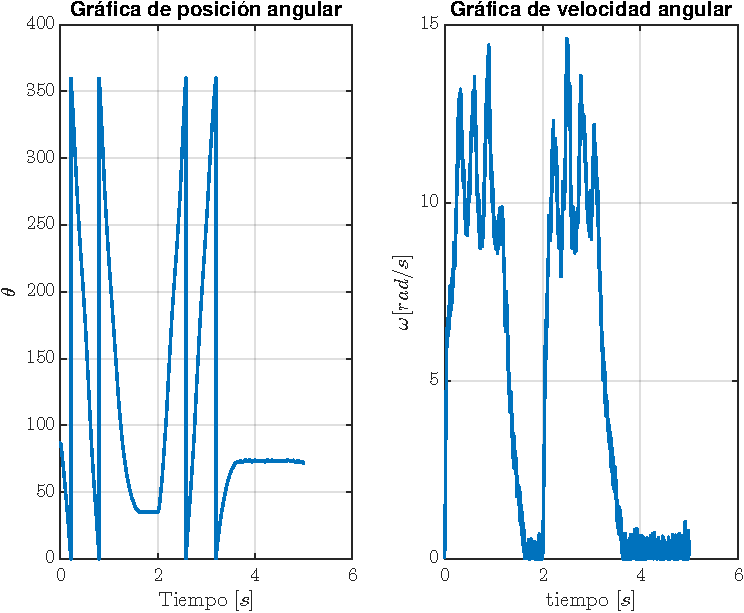
\includegraphics[width=.95\linewidth]{CHPTRS/CH07_IMPLEMENTACION/Fig/w_JGA25.pdf}
        \end{subfigure}
        \\ 
        % FILA-2 (CAPTIONS + LABELS)
        \begin{subfigure}[t]{0.9\linewidth}
            \caption{Respuesta de velocidad angular del motor JGB37 ante señal de prueba.}
            \label{fig:omega_jgb37}
        \end{subfigure}
        &
        \begin{subfigure}[t]{0.9\linewidth}
            \caption{Respuesta de velocidad angular del motor JGA25 ante señal de prueba.}
            \label{fig:omega_jga25}
        \end{subfigure}
    \end{tabularx}
    \caption{Curvas experimentales de velocidad angular registradas durante el sensado.}
    \label{fig:velocidades_prueba}
\end{figure}

\section{Pruebas con la interfaz}
\noindent
En esta sección se muestran las interacciones básicas del usuario con la interfaz desarrollada. En primer lugar, como se mencionó en el Capítulo \ref{ch:CH06} es necesario que el usuario identifique correctamente el puerto de comunicación al que se encuentra conectado el microcontrolador, ya que la transmisión de datos entre la interfaz y el microcontrolador depende directamente de esta configuración.
\noindent
La Figura \ref{fig:acceso_com} muestra,  cómo acceder a la información del sistema para identificar el puerto asignado y copiar el valor correspondiente. Mientras que en la Figura \ref{fig:error_com} se presenta el mensaje de error que aparece cuando se ingresa un puerto incorrecto o inválido, impidiendo la comunicación entre la interfaz y el microcontrolador.

\begin{figure}[!ht]
    \begin{tabularx}{\linewidth}{*{2}{>{\centering\arraybackslash}X}}
        % FILA-1 (IMÁGENES)
        \begin{subfigure}[t]{0.45\textwidth}
            \centering
            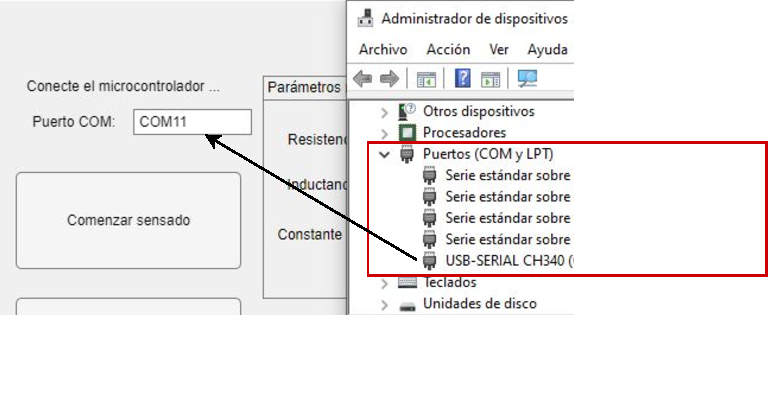
\includegraphics[width=.95\linewidth]{CHPTRS/CH07_IMPLEMENTACION/Fig/1_COM.pdf}
        \end{subfigure}
        &
        \begin{subfigure}[t]{0.45\textwidth}
            \centering
            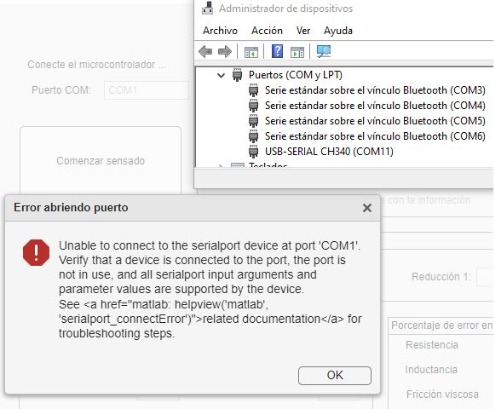
\includegraphics[width=.95\linewidth]{CHPTRS/CH07_IMPLEMENTACION/Fig/2_ERROR_COM.jpg}
        \end{subfigure}
        \\
        % FILA-2 (CAPTIONS + LABELS)
        \begin{subfigure}[t]{0.9\linewidth}
            \caption{Identificación del puerto de comunicación asignado al microcontrolador.}
            \label{fig:acceso_com}
        \end{subfigure}
        &
        \begin{subfigure}[t]{0.9\linewidth}
            \caption{Mensaje de error mostrado al ingresar un puerto incorrecto.}
            \label{fig:error_com}
        \end{subfigure}
    \end{tabularx}
    \caption{Configuración inicial del puerto de comunicación.}
    \label{fig:puerto_com}
\end{figure}
\noindent
Posteriormente, la interfaz validará que el usuario haya completado correctamente los datos de entrada, tales como los parámetros reales de la hoja de datos, si se dispone de ellos, y la indicación de si el motor cuenta o no con caja reductora. En caso contrario, se presentan mensajes de advertencia como el mostrado en la Figura \ref{fig:errores_entrada}.

\begin{figure}[!ht]
    \centering
    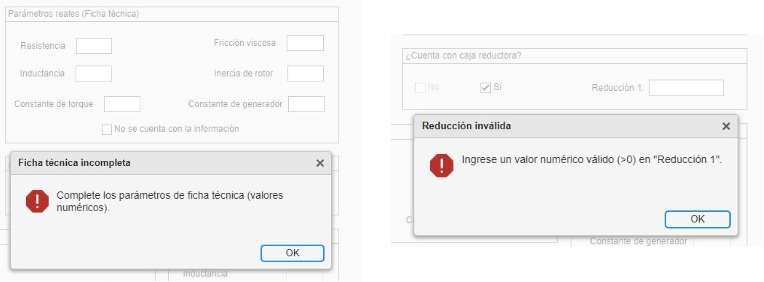
\includegraphics[width=0.7\textwidth]{CHPTRS/CH07_IMPLEMENTACION/Fig/3_ERRORES_INGRESO.jpg}
    \caption{Mensaje de advertencia cuando no se completan los datos requeridos por la interfaz.}
    \label{fig:errores_entrada}
\end{figure}
\noindent
Una vez configurado correctamente el puerto y completados los datos requeridos, se procede a iniciar el sensado. La Figura \ref{fig:sensado_correcto} muestra el funcionamiento adecuado de la comunicación entre la interfaz y el microcontrolador, donde se grafican en tiempo real las variables medidas del motor.

\begin{figure}[!ht]
    \centering
    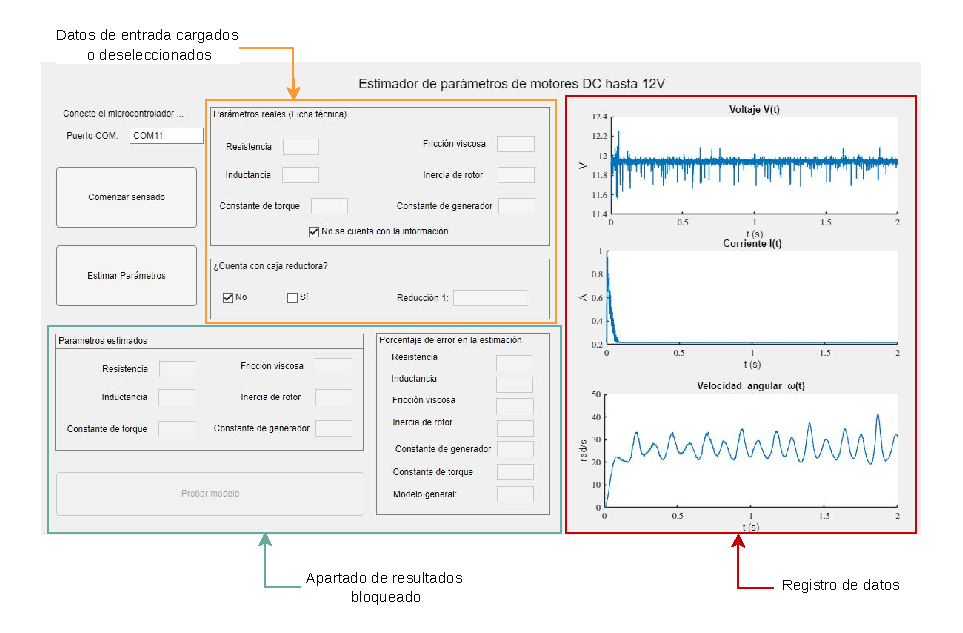
\includegraphics[width=0.9\textwidth]{CHPTRS/CH07_IMPLEMENTACION/Fig/4_FUNCIONAMIENTO-SENSADO.drawio.pdf}
    \caption{Visualización en tiempo real de las variables medidas durante el proceso de sensado.}
    \label{fig:sensado_correcto}
\end{figure}
\noindent
Luego de verificar que los datos adquiridos son coherentes, el usuario puede proceder a estimar los parámetros del motor. Para mayor detalle sobre el algoritmo utilizado, puede consultarse el Anexo \ref{an:Anexo_C}. La Figura \ref{fig:estimacion_resultados} muestra los resultados obtenidos tras ejecutar la estimación.

\begin{figure}[!ht]
    \centering
    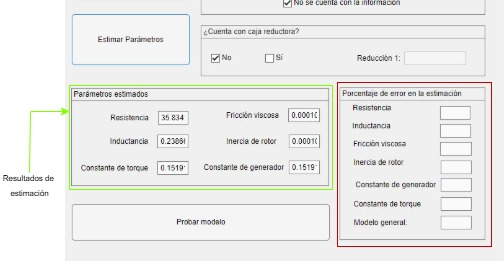
\includegraphics[width=0.9\textwidth]{CHPTRS/CH07_IMPLEMENTACION/Fig/5_Resultados.jpg}
    \caption{Resultados de la estimación paramétrica mostrados en la interfaz.}
    \label{fig:estimacion_resultados}
\end{figure}
\noindent
Si bien la interfaz cumple su función de presentar los resultados en las casillas respectivos, puede mejorarse en futuras iteraciones incorporando explícitamente las unidades correspondientes en el \ac{SI} junto a cada parámetro estimado, ya que no queda tan claro en qué unidades está la dimensional de los resultados, para saber las unidades de estos parámetros, esta información puede consultar en en el Anexo \ref{an:Anexo_E}.
\noindent
Posteriormente de presentar los resultados, se habilita la opción de probar el modelo con los parámetros estimados. En esta etapa se carga en el microcontrolador una rutina descrita en el Capítulo \ref{ch:CH06}, destinada a realizar una nueva toma de datos para la validación del modelo. Con los parámetros previamente estimados se construye un modelo ideal de la planta, cuya respuesta se grafica junto a las señales medidas, como se observa en la Figura \ref{fig:prueba_modelo}.

\begin{figure}[!ht]
    \centering
    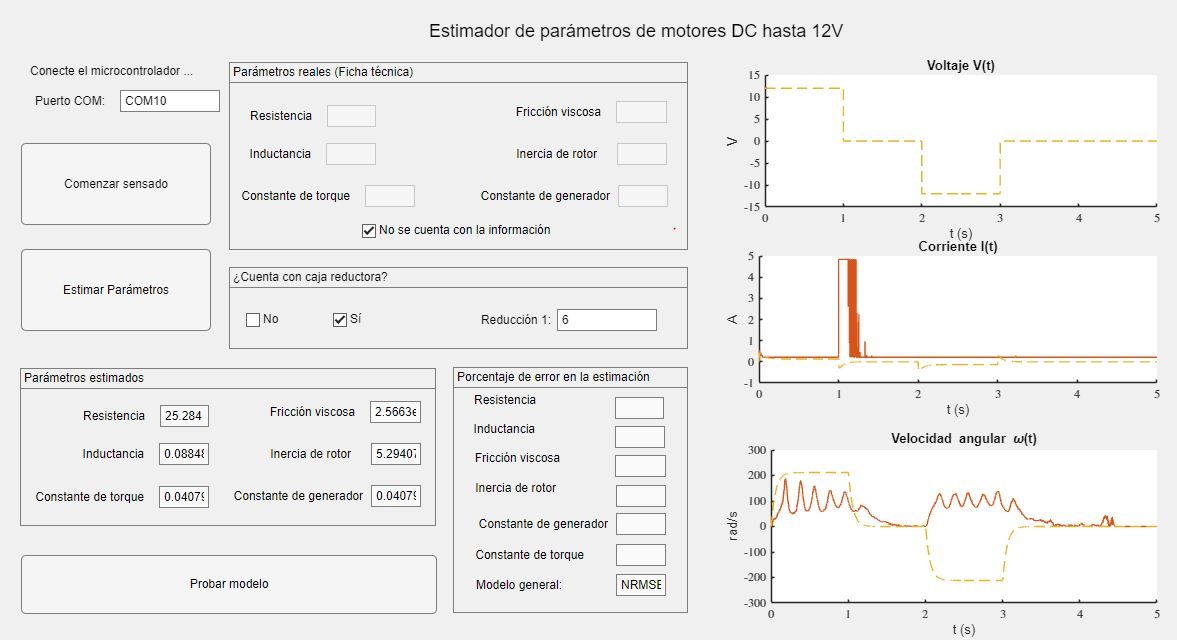
\includegraphics[width=0.9\textwidth]{CHPTRS/CH07_IMPLEMENTACION/Fig/6_Discución_final.JPG}
    \caption{Comparación entre la respuesta experimental y el modelo ideal construido con los parámetros estimados.}
    \label{fig:prueba_modelo}
\end{figure}
\noindent
Finalmente, durante las pruebas se identificó un comportamiento particular en el sensado. En el caso de la velocidad angular, se observa una oscilación alrededor de un punto de operación, lo cual indica la necesidad de aplicar un filtrado adicional para mejorar la calidad de la señal. Asimismo, en el sensado de corriente se evidencia un pico significativo cuando el motor es forzado a detenerse, tal como se aprecia en la Figura \ref{fig:pico_corriente}.

\begin{figure}[!ht]
    \centering
    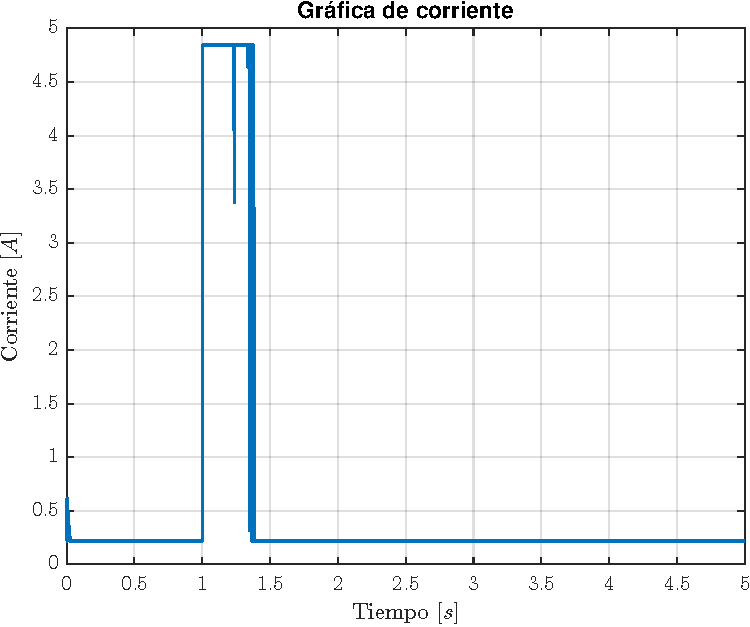
\includegraphics[width=0.9\textwidth]{CHPTRS/CH07_IMPLEMENTACION/Fig/7_Ayuda_discución_final.pdf}
    \caption{Pico de corriente registrado al forzar la detención del motor.}
    \label{fig:pico_corriente}
\end{figure}
\noindent
Este fenómeno sugiere que parte de la información podría no estar siendo capturada correctamente por el micrcontrolador. Como se mencionó en la sección \ref{sec:pruebas_driver}, se emplea una ganancia genérica para escalar la medición de corriente del motor. Es posible que esta configuración esté provocando saturación en el ADC del microcontrolador, impidiendo una medición precisa en condiciones transitorias abruptas. Este efecto introduce uu arrastre de error en el proceso de estimación y deberá analizarse con mayor detalle en futuras iteraciones del sistema.

